\documentclass{beamer}
\let\vec\mathbf
\mode<presentation>
\usepackage{amsmath}
\usepackage{amssymb}
%\usepackage{advdate}
\usepackage{adjustbox}
%\usepackage{subcaption}
\usepackage{enumitem}
\usepackage{multicol}
\usepackage{mathtools}
\usepackage{listings}
\usepackage{url}
\usetheme{Boadilla}
\usecolortheme{lily}
\setbeamertemplate{footline}
{
  \leavevmode%
  \hbox{%
  \begin{beamercolorbox}[wd=\paperwidth,ht=2.25ex,dp=1ex,right]{author in head/foot}%
    \insertframenumber{} / \inserttotalframenumber\hspace*{2ex} 
  \end{beamercolorbox}}%
  \vskip0pt%
}
\setbeamertemplate{navigation symbols}{}
\providecommand{\nCr}[2]{\,^{#1}C_{#2}} % nCr
\providecommand{\nPr}[2]{\,^{#1}P_{#2}} % nPr
\providecommand{\mbf}{\mathbf}
\providecommand{\pr}[1]{\ensuremath{\Pr\left(#1\right)}}
\providecommand{\qfunc}[1]{\ensuremath{Q\left(#1\right)}}
\providecommand{\sbrak}[1]{\ensuremath{{}\left[#1\right]}}
\providecommand{\lsbrak}[1]{\ensuremath{{}\left[#1\right.}}
\providecommand{\rsbrak}[1]{\ensuremath{{}\left.#1\right]}}
\providecommand{\brak}[1]{\ensuremath{\left(#1\right)}}
\providecommand{\lbrak}[1]{\ensuremath{\left(#1\right.}}
\providecommand{\rbrak}[1]{\ensuremath{\left.#1\right)}}
\providecommand{\cbrak}[1]{\ensuremath{\left\{#1\right\}}}
\providecommand{\lcbrak}[1]{\ensuremath{\left\{#1\right.}}
\providecommand{\rcbrak}[1]{\ensuremath{\left.#1\right\}}}
\theoremstyle{remark}
\newtheorem{rem}{Remark}
\newcommand{\sgn}{\mathop{\mathrm{sgn}}}

\providecommand{\res}[1]{\Res\displaylimits_{#1}} 
\providecommand{\norm}[1]{\lVert#1\rVert}
\providecommand{\mtx}[1]{\mathbf{#1}}

\providecommand{\fourier}{\overset{\mathcal{F}}{ \rightleftharpoons}}
%\providecommand{\hilbert}{\overset{\mathcal{H}}{ \rightleftharpoons}}
\providecommand{\system}{\overset{\mathcal{H}}{ \longleftrightarrow}}
	%\newcommand{\solution}[2]{\textbf{Solution:}{#1}}
%\newcommand{\solution}{\noindent \textbf{Solution: }}
\providecommand{\dec}[2]{\ensuremath{\overset{#1}{\underset{#2}{\gtrless}}}}
\newcommand{\myvec}[1]{\ensuremath{\begin{pmatrix}#1\end{pmatrix}}}

\title{Matrices in Geometry - 2.4.32}
\author{EE25BTECH11035  Kushal B N}
\date{Sep, 2025}

\begin{document}

\maketitle


\begin{frame}
\tableofcontents
\end{frame}

\section{Problem Statement}
\begin{frame}
\frametitle{Problem Statement}
The points $\vec{A}\brak{-1,-2}$, $\vec{B}\brak{4,3}$, $\vec{C}\brak{2,5}$ and $\vec{D}\brak{-3,0}$ in that order form a rectangle.
\end{frame}

\section{Solution}
\begin{frame}{Solution}
   Given $\vec{A}\myvec{-1\\-2}$, $\vec{B}\myvec{4\\3}$, $\vec{C}\myvec{2\\5}$ and $\vec{D}\myvec{-3\\0}$. \\
   
 \begin{equation}
\vec{B} - \vec{A} = \myvec{5\\5}
\end{equation}

\begin{equation}
\vec{C} - \vec{B} = \myvec{-2\\2}
\end{equation}

\begin{equation}
\vec{D} - \vec{C} = \myvec{-5\\-5}
\end{equation}

\begin{equation}
\vec{A} - \vec{D} = \myvec{2\\-2}
\end{equation}
    
\end{frame}



\begin{frame}{Solution}
Checking opposite sides,\\
\begin{equation}
\brak{\vec{B} - \vec{A}} = - \brak{\vec{D} - \vec{C}}
\end{equation}

Now, as each pair of opposite sides are parallel and equal in length, this means that the given points make up a parallelogram.\\

Checking for right angle, we need to check for inner product of the adjacent sides of the parallelogram.\\

\begin{equation}
\brak{\vec{B}-\vec{A}}^{\top}\brak{\vec{C}-\vec{B}} = \myvec{5 & 5}\myvec{-2\\2} = 0
\end{equation}

This implies that the angle at B is a right angle. A parallelogram with a right angle is a rectangle.

\end{frame}

\begin{frame}{Solution}
Checking for square:\\
The given quadrilateral will be a square if its diagonals are orthogonal.

\begin{equation}
    \brak{\vec{C}-\vec{A}}^{\top}\brak{\vec{D}-\vec{B}} = \myvec{3&7}\myvec{-7\\-3} = -42
\end{equation}

From $\brak{7}$, we can see that $\brak{\vec{C}-\vec{A}}^{\top}\brak{\vec{D}-\vec{B}} \neq 0$, that is the diagonals are not orthogonal and hence the given quadrilateral cannot be a square.\\
Hence, it is proved that the given points $\vec{ABCD}$ in that order form a rectangle.

\end{frame}

\section{Conclusion}
\begin{frame}{Conclusion}
$\therefore$ The quadrilateral $\vec{ABCD}$ is a rectangle.

\begin{figure}
    \centering
    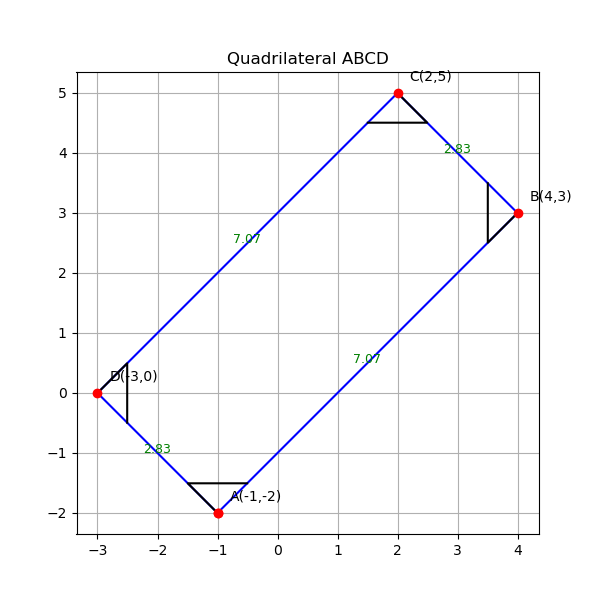
\includegraphics[width=0.65\columnwidth]{figs/1.png}
\end{figure}

\end{frame}
\end{document}